\documentclass[border=10pt]{standalone}

\usepackage{tikz}
\usepackage{tikzsymbols}
\usetikzlibrary{calc,patterns,shapes.geometric}

\def\centerarc[#1](#2)(#3:#4:#5){\draw[#1] ($(#2)+({#5*cos(#3)},{#5*sin(#3)})$) arc (#3:#4:#5);}

\begin{document}
	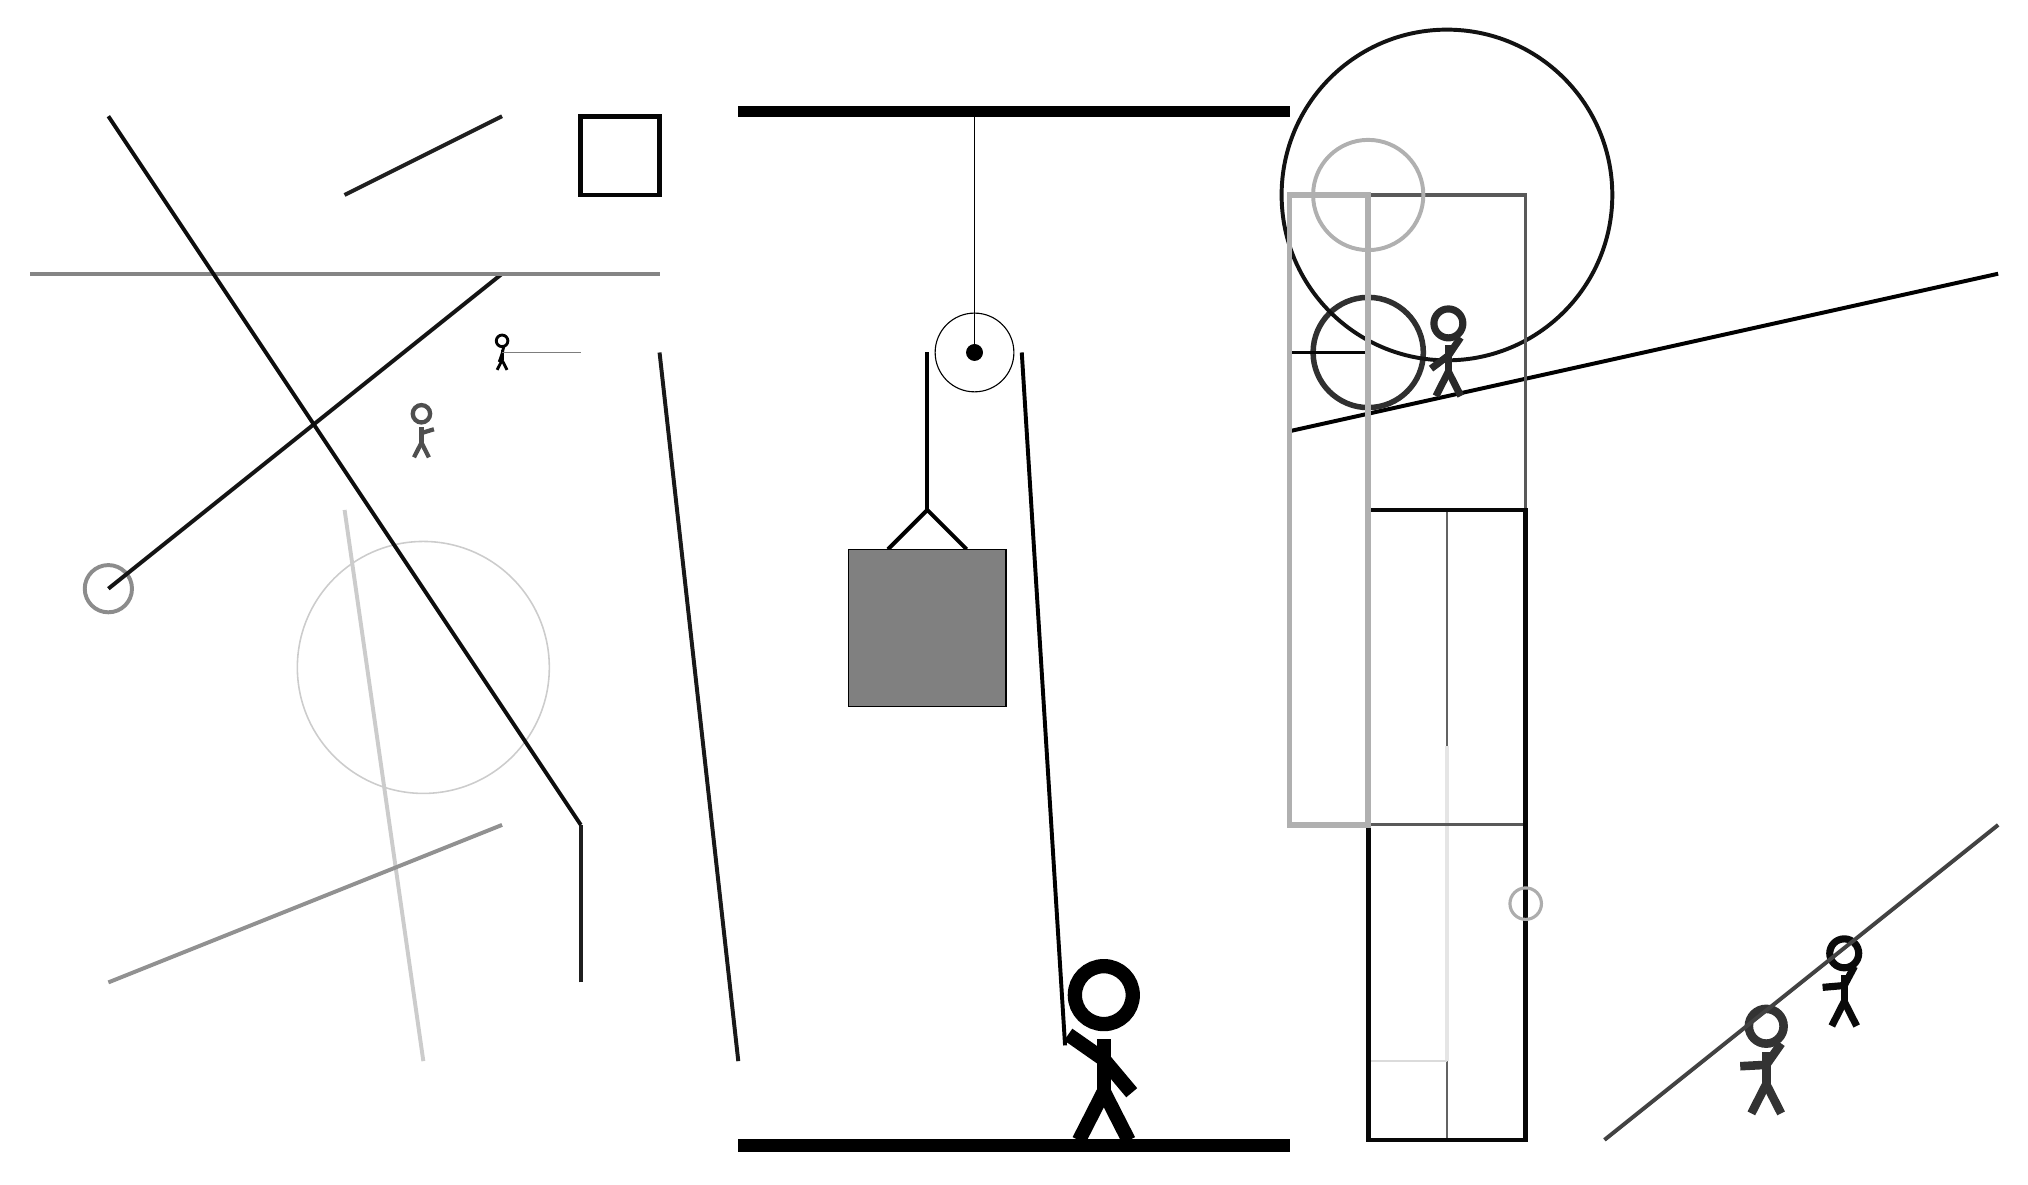
\begin{tikzpicture}
		%%%%% START %%%%%
		
		\draw[fill=black] (-2, 10) rectangle (5, 10.125);
		
		\draw (1, 7) circle (0.5);
		\draw[fill=black] (1, 7) circle (0.1);
		\draw (1, 10) -- (1, 7);
		
		\node[line width=0.3mm, color=black!96] at (12, -1) {\Strichmaxerl[5][5][62]};
		
		\draw [line width=0.5mm, color=black!45](-10, 4) circle (0.3);
		\draw[line width=0.5mm, color=black!81](7, 2) -- (7, 0);
		\node[line width=0.5mm, color=black!80] at (11, -2) {\Strichmaxerl[6][3][55]};
		\draw[line width=0.5mm, color=black!88](-4, -1) -- (-4, 1);
		\draw[line width=0.5mm, color=black!74](9, -3) -- (14, 1);
		\node[line width=0.2mm, color=black!99] at (-5, 7) {\Strichmaxerl[2][71][77]};
		
		\draw[line width=0.5mm, color=black!100](5, 6) -- (14, 8);
		\node[line width=0.7mm, color=black!69] at (-6, 6) {\Strichmaxerl[3][90][17]};
		\draw[line width=0.2mm, color=black!61] (6, -3) rectangle (7, 5);
		
		\draw[line width=0.4mm, color=black!10] (7, -2) rectangle (7, 2);
		\draw[line width=0.5mm, color=black!90](-2, -2) -- (-3, 7);
		\draw [line width=0.7mm, color=black!81](6, 7) circle (0.7);
		
		\draw[line width=0.5mm, color=black!92](-5, 8) -- (-10, 4);
		\draw[line width=0.5mm, color=black!20](-6, -2) -- (-7, 5);
		\draw [line width=0.5mm, color=black!93](7, 9) circle (2.1);
		
		\draw[line width=0.5mm, color=black!48](-3, 8) -- (-11, 8);
		\draw[line width=0.4mm, color=black!98] (6, 7) rectangle (5, 9);
		\draw[line width=0.2mm, color=black!14] (6, -2) rectangle (7, -2);
		
		\draw [line width=0.2mm, color=black!20](-6, 3) circle (1.6);
		\draw[line width=0.4mm, color=black!65] (6, 9) rectangle (8, 1);
		\draw[line width=0.5mm, color=black!88](-7, 9) -- (-5, 10);
		\draw[line width=0.5mm, color=black!95](-4, 1) -- (-10, 10);
		\draw[line width=0.6mm, color=black!97] (6, 5) rectangle (8, -3);
		\draw[line width=0.7mm, color=black!31] (5, 1) rectangle (6, 9);
		
		\node[line width=0.7mm, color=black!84] at (7, 7) {\Strichmaxerl[5][37][56]};
		
		\draw [line width=0.5mm, color=black!31](6, 9) circle (0.7);
		\draw[line width=0.6mm, color=black!98] (-3, 9) rectangle (-4, 10);
		\draw[line width=0.5mm, color=black!43](-5, 1) -- (-10, -1);
		\draw [line width=0.4mm, color=black!32](8, 0) circle (0.2);
		\draw[line width=0.2mm, color=black!51] (-4, 7) rectangle (-5, 7);
		
		
		\draw[line width=0.5mm] (-0.1, 4.5) -- (0.4, 5.0) -- (0.9, 4.5);
		\draw[fill=black!50] (-0.6, 4.5) rectangle (1.4, 2.5);
		
		\draw[line width=0.5mm] (0.4, 7) -- (0.4, 5.0);
		\centerarc[line width=0.5mm](1, 7)(0:180:0.6);
		\draw[line width=0.5mm](1.6, 7) -- (2.15, -1.8);
		
		\node at (2.6, -1.9) {\Strichmaxerl[10][-35][-50]};
		
		\draw[fill=black] (-2, -3) rectangle (5, -3.15);
		
		%%%%% END %%%%%
	\end{tikzpicture}
\end{document}